\documentclass[11pt,a4paper]{article}
\usepackage{od}
\usepackage[utf8]{inputenc}
\usepackage[main=german,russian]{babel}

\title{Das Tätigkeits-Natur-System} 

\author{Piotr Georgievich Shchedrovitsky}
\date{10.11.2012}

\begin{document}
\maketitle
\begin{quote}
  Übersetzt von Hans-Gert Gräbe, Leipzig.
  
  Quelle: \foreignlanguage{russian}{Пётр Щедровицкий. Деятельностно-природная
    система. Журнал «Человек и природа». — М., «Знание», 1987, № 12,
    с. 12–63}.  Digitale Publikation unter
  \url{https://gtmarket.ru/laboratory/expertize/5412}
\end{quote}

\tableofcontents
\clearpage

Piotr Georgievich Shchedrovitsky ist ein russischer Philosoph, Methodologe,
Gründer und Leiter der Schule für Kulturpolitik. Er absolvierte die Fakultät
für Pädagogik und Psychologie am Moskauer Staatlichen Pädagogischen Institut,
arbeitete an Fragen der Psychologie, der Managementmethodik, der Organisation
angewandter komplexer Forschung in verschiedenen Bereichen (Pädagogik,
Management, Rohstoff\-förderung) sowie auf dem Gebiet der Umweltbildung und
der Ausarbeitung von Umweltprogrammen auf der Grundlage methodischer Forschung
Forschungen.  Er hat dazu beigetragen, dass Begriffe wie „Kulturpolitik“,
„Russische Welt“, „Humanity-Technologien“ (zusammen mit E. Ostrovsky),
"geoökonomisches Gleichgewicht“ (zusammen mit V. Knyaginin),
„Anthropostrukturen“ und „Anthropoströme“ (zusammen mit S.  Gradirovsky) in
moderne Diskussionen Eingang gefunden haben. Er entwickelte Vorstellungen von
Framing-Techniken des Denkens und den ressourcenbasierten Ansatz konsequent
weiter. Er hat eine Reihe von Politikern, Parteien und staatlichen
Institutionen beraten.  Er war an der Erstellung von Entwicklungsstrategien
für eine Reihe russischer Regionen beteiligt.  Der hier vorgestellte Text
wurde erstmals 1987 veröffentlicht.

\section{Einleitung}

Die Situation, die sich im letzten Viertel des zwanzigsten Jahrhunderts in
Gebieten und Tätigkeitsbereichen herausgebildet hat, in denen das Material der
Natur für menschliche Bedürfnisse erfasst und ausgenutzt wird, zwingt
Ideologen und Theoretiker, Organisatoren und Ingenieure, den sich in
Jahrhunderten herausgebildeten Korpus theoretischer und praktisch-methodischer
Ansätze zu einem großen Teil zu überdenken und zu revidieren: Technik und
Wissenschaft, Engineering und Lebensstile -- alle steht unter ökologischem
Zweifel. Viele gewohnte Handlungs- und Denkweisen müssen heute verworfen
werden.  Der produktive und konsumtive Enthusiasmus des zivilisierten Menschen
muss begrenzt werden. Die gewohnte Strategie des extensiven Wachstums
kollidiert mit einem ökologisch orientierten gesellschaftlichen Bewusstsein.

Was aber wird eigentlich die bestehenden Prinzipien der Organisation und
Leitung der sozialen Produktion ersetzen? Was sind die Perspektiven der
Entwicklung des Komplexes der Projeksteuerung und der Energetik? Was sind die
perspektivischen Linien der Entfaltung einer regionale ökologischen Politik?
Wie muss das Ingenieursdenken beschaffen sein, das abfallfreie und ökologische
Technologien schafft?

Es ist klar, dass es auf diese Fragen keine eindeutigen und vollständigen
Antworten gibt.  Gleichzeitig verstehen wir, dass die richtige
\emph{Formulierung der Frage} bereits die halbe Antwort ist.  Es ist
wichtiger, die Problemsituation zu skizzieren als eine bis zur letzten
Nachkommastelle korrekte Antwort auf eine Frage zu geben, die grundlegend
falsch gestellt ist. Um jedoch ein Gefühl für die tiefliegenden Probleme zu
bekommen und die Hauptfragen herauszuarbeiten, sind \emph{neue Konzepte und
  Vorstellungen} erforderlich, auf die sich das Denken im Prozess der
Problematisierung, der Suche nach neuen Ansätzen und neuen Lösungen stützen
kann.  Ehe die einen oder anderen Projekte vorgeschlagen werden, muss ein
angemessener konzeptioneller Apparat gebildet werden, jene Sprache, in der
ökologische Programme und ökologische Aspekte der Entwicklung von sozialen
Systemen besprochen werden können.

Um die Problematik zu öffnen und die notwendigen Vorstellungen in der
notwendigen Weise zu umreißen, muss man sich der vorhandenen soziokulturellen
Situation zuwenden, müssen die Tendenzen der Änderung von Tätigkeitsbereichen
herausarbeiten, die sich herausgebildet haben und das Gesicht der sozialer
Systeme prägen, muss die Grenzen der Situation selbst als problematische
ökologische Situation abstecken.

Dabei beginnen wir unsere Analyse mit konkreten Tätigkeitsbereichen und
-feldern, betrachten private und lokale Schwierigkeiten und Paradoxien im
weiteren Sinne und ordnen sie ein als Manifestation allgemeiner Tendenzen des
Funktionierens und der Entwicklung von natürlich-technischen und
Tätigkeits-Natur-Systemen.

\section{Extraktive Technologien: Bedingungen, Lage der Dinge, Situation}

Wenden wir uns den Erfahrungen des Managements in der extraktiven Industrie
zu.  Der Verzicht auf primitive Zugänge und Technologien, die schnelle Effekte
für genügend einfache, oberflächennahe Lagerstätten versprechen, die
Notwendigkeit der Koordinierung verschiedener Infrastrukturen innerhalb der
Rohstoffindustrie unter Hinzunahme breiterer wirtschaftlicher Mechanismen --
all das rückt heute Aufgaben von Organisation, Leitung und Steuerung im
weitesten Sinne in den Vordergrund. Die fallende Abbauergiebigkeit, zunehmende
Schwierigkeiten der geologischen und bergbaulichen Bedingungen der Gewinnung
von Bodenschätzen bleiben nicht ohne Auswirkungen auf die Vergrößerung der
organisatorischen Strukturen in der Rohstoffindustrie; die Kompliziertheit der
Systeme spiegelt sich direkt im Charakter der Organisations- und
Managementarbeit wider. Bisher hat diese Änderung jedoch auf die extensiven
Parameter ausgewirkt -- die Frage der Qualität der Organisations- und
Managementarbeit wird nicht direkt gestellt und zieht keine Aufmerksamkeit auf
sich.  Aus unserer Sicht ist es heute notwendig, nicht nur den Stil, sondern
auch den gesamten Organisations- und Managementansatz in der Rohstoffindustrie
grundlegend zu ändern.

Als Beispiel können wir uns auf die Situation innerhalb der Öl- und
Gasindustrie konzentrieren. Die erste Frage, die man sich stellen muss, wenn
man eine Analyse der Organisation- und Managementstrukturen dieser Sphäre
beginnen will, ist, welche Prozesse sind Führungsprozesse und gleichzeitig, in
welchem Rahmen muss das Objekt und dedr Gegenstand der Managementprozesse
beschrieben werden?  Etwa ist die Frage zu klären, ob die Förerung von Öl und
Gas ein produktiver oder ... ein Transportprozess ist.

Diese Frage ist grundlegend: Methoden und Formen des Managements in den beiden
Fällen unterscheiden sich grundlegend voneinander. Wenn wir davon ausgehen,
dass die Förderung von Öl und Gas ein Produktionsprozess ist, dann ist es
natürlich zu fragen, was produziert wird und was das Produkt dieser Produktion
ist. Auf diese Frage kann schon nicht mehr geantwortet werden: Öl und Gas. Öl
oder Gas selbst sind kein Produkt der Produktion; sie sind als Halbzeug oder
Primärrohstoff für einen Produktionsprozess zu betrachten, der über die
Extraktion hinausgeht.

Mit anderen Worten: Die Gewinnung oder Förderung von Öl und Gas selbst ist
kein Produktionsprozess. Außerdem, je nachdem, in welche größeren
organisatorischen und wirtschaftlichen Strukturen der Extraktionsprozess
eingeschlossen ist, wird er verschiedene Funktionen und verschiedene
organisatorische Belastungen haben. Wenn das geförderte Öl durch Pipelines ins
Ausland geschickt wird, dann ist die Förderung ein Teil eines Transportsystems
oder ein Teil des Außenhandels. Wird das geförderte Öl hingegen zu anderen
Produkten verarbeitet, wird die Förderung zu einem Teil des Transportsystems
oder zu einem Fragment des Außenhandels.  Wird es hingegen zu anderen
Produkten verarbeitet, so wird die Extraktion zu einem Teil eines
Produktionsprozesses.

Diese elementare Grammatik des Managements bewegt jedoch die Organisatoren in
den extraktiven Industrien in keiner Weise. Ohne über die Folgen und
Perspektiven ihrer Wahl der einen oder anderen Organisationsstrategie
nachzudenken, setzen sie naiv voraus, dass die Förderung von Öl und Gas selbst
ein eigenständiger Produktionsprozess ist, und verwenden alle sekundären
Methoden der organisatorischen und wirtschaftliche Analysen, welche die
Effektivität und die „wirtschaftlichen“ Vorteile des gewählten Ansatzes zeigen
sollen.

Nur ein radikaler Bruch mit bestehenden Stereotypen und druch äußere
Einwirkung bewirken, dass die Organisatoren beginnen, die Situation zu
reflektieren. Der Verfall der Ölpreise auf dem Weltmarkt zeigt zum ersten Mal,
dass der Verkauf weder effizient noch profitabel ist. Es stimmt, dass bereits
im 13. Jahrhundert die einfache merkantilistische Weisheit formuliert wurde,
dass es profitabler ist, verarbeitete Waren zu verkaufen als der Verkauf von
Rohstoffen. Aber die Festigkeit etablierter Verwaltungsprinzipien ist stärker
als merkantilistische Weisheit. Es ist nun notwendig, die übliche Strategie
aufzugeben und eine wirklich organisatorische Managementaufgabe zu lösen: was
und wie soll produziert werden?

Übrigens ist diese Frage alles andere als trivial. Alle Nebenprodukte sind ein
Moment und Fragment innerhalb des Brennstoff-Energie-Komplexes und damit ein
Moment des Systems der gesellschaftlichen Reproduktion. Mit anderen Worten,
wenn wir Benzin und Heizöl produzieren, produzieren wir es natürlich, aber
Sinn erhält diese Produktion erst im Rahmen eines größeren Systems -- wiederum
eine einfache Systemweisheit.

Aber dann, wenn man mit der Organisations- und Managementanalyse fortfährt,
ist es natürlich zu fragen: Welches Gewicht und welchen Status hat die
Förerung von Öl und Gas im Rahmen des Brennstoff-Energie-Komplexes?  Wenn die
Frage so gestellt wird, müsste der Organisator anfangen nachzudenken. Er würde
ein Stück Papier und einen Stift nehmen und zunächst einmal alles zählen, was
den Brennstoff-Energie-Komplex des Landes ausmacht.  Kernkraft, Wasserkraft,
Kohle, Öl und Gas, Solar- und Wasserkraftwerke, neue Motoren und neue
Autodesigns, neue Arten von Rahmen und Fensterglas ... Mit einer solch
einfachen Aufzählung kann eine Reihe von komplexen Forschungs- und
Entwicklungsprogrammen initiiert werden, die auf eine Verringerung des Gewicht
der Förderung und des Verbrauchs von Öl und Gas innerhalb des
Brennstoff-Energie-Komplexes gerichtet sind, um diesen wertvollsten Rohstoffe
aus den bestehenden Mechanismen der nicht-rationalen Nutzung herauszulösen und
in den Rahmen des chemisch-rohstofflichen Komplexes zu verschieben.

Die gleiche einfache merkantilistische Weisheit zeigt, dass es wesentlich
effizienter ist, auf der Basis von Erdölprodukten Medikamente herzustellen als
Heizöl. Mit anderen Worten, man könnte die Extraktionstechnologie nicht in den
Rahmen der Reproduktion und brennstoff-energetischen Absicherung des
Wirtschaftsmechanismus einordnen, sondern in die Rahmen der Entwicklung und
Schaffung neuer Biotechnologien und Heilpräparate.

Wenn man anerkennt, dass die Rohstoffindustrie heute ein sehr komplexes
organisatorisch-technischen System bildet, sind wir verpflichtet, die Frage
nach den optimalen organisatorischen \emph{Strategien und Prinzipien}, die
dieser Art von System adäquat sind, auf die Tagesordnung zu setzen. Wir müssen
uns von einer falschen Produktionsideologie verabschieden, nach der sich
herausstellt, dass das geförderte Öl (manchmal 12--15 Prozent der Vorräte, und
noch auf eine solche Weise, dass die verbleibenden 85 Prozent nie extrahiert
werden können) ein Produkt ist, der stoffliche Nachweis der Produktivität.
Wir müssen neue Programme auflegen -- sowohl in bei der Suche nach
alternativen Kraftstoffen (das macht jede Ölfirma im Ausland), als auch im
Bereich prinzipiell neuer Formen der Nutzung von Öl und Erdölprodukten.  Wir
sind heute mit der Notwendigkeit konfrontiert, die Frage neu zu prüfen und zu
lösen, was die prinzipiellen Managementstrategien in der Rohstoffindustrie
sind.  Worauf kann sich der Organisator und Manager stützen, wenn er plötzlich
beschließt, sich von den „großväterlichen“ Zugängen zu den natürlichen
Möglichkeiten der Erde zu verabschieden?

Wir müssen verstehen, dass die Rohstoffindustrie nicht nur ein komplexes
organisatorisch-technisches System ist. Es ist ein organisatorisch-technisches
System auf natürlichem Material. Mit anderen Worten: Die organisatorischen und
technischen Systeme in diesem Bereich \emph{„parasitieren“ auf natürlichem
  Material}, verbrauchen und verarbeiten dieses Material, wirken auf dieses
ein, indem sie jeweils relativ große Zonen und Areale des Territoriums
ausbeuten -- Länder, Wälder und Wasser.

Der Charakter solcher Art von Einwirkungen ist immer sehr schwer vorhersehbar
und gleichzeitig ist es organisatorisch sehr schwierig, echte Grenzen des
Systems zu ziehen, über dessen Management wir sprechen. Tätigkeitsorientierte
(\foreignlanguage{russian}{деятельностные}) und natürliche Momente „leben“ in
verschiedenen Zeiten und folgen verschiedenen Gesetzen, sie sind veschiedener
Logik unterworfen, was bedeutet, dass auch die Zugänge zu ihnen verschieden
sein müssen. Indem diese oder jene für einen gegebenen Tätigkeitstyp führende,
vorherrschende Art von Naturmaterial verbraucht oder verarbeitet wird, wirken
diese Systeme auf ein größeres Areal, transformieren dessen Charakteristiken
wesentlich und verändern damit die Handlungsbedingungen anderer
wirtschaftlicher Infrastrukturen. 

\section{Die ökologische Lage: erste Orientierungspunkte}

Bis vor kurzem hat sich im Managementbereich der Mythos von der
„Unerschöpflichkeit“ der Ressourcen der Erde gehalten. Oftmals, wenn
ökologische Fragen mit wirtschaftlichen Entscheidungsträgern aller Ränge
erörtert wurden -- wie in den extraktiven Industrien so auch in der
Bauindustrie -- hört man Selbstberuhigung: „Das Land ist groß“ ...  Es macht
sich eine jahrzehntelange Tradition von Haltungen und Überzeugungen in Bezug
auf die natürlichen und menschlichen Ressourcen bemerkbar, ein Führungsstil
und die Selbstdefinition eines „Managers auf zwei Jahre“ -- eines Managers auf
Zeit. 

In den letzten Jahrzehnten hat das Ausmaß des anthropogenen und technogenen
Einflusses auf die Umwelt soclhe Maßstäbe erreicht, dass der gesamte Planet
und das Leben selbst auf ihm gefährdet ist. Immer mehr Spezialisten, breitere
Gruppen der Öffentlichkeit diskutieren und analysieren die ökologische
Situation, wie sie sich in verschiedenen Bereichen, Tätigkeitsfeldern und
geografischen Zonen entwickelt hat. Die Problematik der Ökologie ist auf der
Prioritätenliste nationaler Themen ganz nach oben gerückt. Alle sprechen über
Ökologie, die Umweltbewegung nimmt Fahrt auf, deren Vertreter beharren auf
einer grundlegenden Änderung der bestehenden technologischen und
organisatorischen Strategien und individueller Lösungen.

Allerdings weiß niemand wirklich, was das ist -- Ökologie, und was die
Prinzipien und Ansätze sind, auf die sich ein neues -- ökologisches -- System
des Wirtschaftens stützen soll.  Das erste, womit man unmittelbar konfrontiert
ist und worauf das ökologische Bewusstsein drängt, das ist der Fakt der
unberücksichtigten und unkontrollierbaren Folgen von technogenen Einwirkungen
auf die natürliche Umwelt.  Indem man es mit komplizierten Tätigkeitssystemen
zu tun hat, die auf Naturmaterial parasitieren, befinden wir uns ständig in
der Situation des Auseinanderfallens, des „Zerreißens“ zwischen den
Handlungszielen und den tatsächlichen Folgen und Ergebnisse dieser Handlungen.
Das Fehlen einer adäquaten Vorstellung vom „Leben“ der Natur unter technogenen
Einwirkungen macht sich sofort bemerkbar, wenn wir über die Grenzen von
Prinzipien und Maßstäben der Einflussnahme auf die Natur, die sich über
Jahrhunderte bewährt haben, hinausgehen.

Die realen Folgen weichen stark von den Erwartungen und Prognosen ab, Folgen
von Sekundärmaßnahmen zur Kompensation der ursprünglichen Folgen weichen
wiederum von den Zielen ab, und... so weiter. Die Folgen nehmen einen
lawinenartigen unkontrollierbaren Charakter an, und wir leben faktisch in
einer Welt der „Nachbehandlungen“ unserer eigenen Züge, in einer künstlichen,
von uns erdachten und erschaffenen Welt. Ein Unglück kommt hinzu: auf den uns
umgebenden Erscheinungen und Kataklysmen kann niemand Schilder mit Hinweisen
und Preisen anbringen, wer, wann und wie diese Folgen hervorgerufen hat, für
die wir im Prinzip „zahlen“, und wie lange wir nch gezwungen  sind zu zahlen.  

Das Ausmaß dieser Erscheinungen ist wirklich katastrophal, wir haben es mit
einer breiten ökologische Situation zu tun, die viele Ideologen, Theoretiker
und gesellschaftlich Tätige vollkommen zu recht als Situation einer
ökologischen Krise bezeichnen und nicht mit apokalyptischen Prognosen sparen.

Es ist schwierig, auf die Fragen zu antworten: Wie können wir die Auswirkungen
unsseres Handelns erfassen und kontrollieren, was müssen wir tun, um eine
ökologische Katastrophe abzuwenden, und woran muss ein Organisator denken, der
es mit dieser Art von heterogenen und heterarchisierten Systemen zu tun hat,
die sowohl Tätigkeits- als auch natürliche Komponenten umfassen?

Wo, in welchem Wissensgebiet können wir nach Antworten auf diese Fragen
suchen? Fakt ist, dass wir die ökologische Situation nicht ignorieren können.
Fakt ist auch, dass nicht bekannt ist, wie sie berücksichtigen. In den letzten
Jahren sprechen wir über \emph{rationale Naturnutzung}, über Strategien der
Ressourcenschonung, über rationale Territorialerschließung. Entfernt man
jedoch das Wort „rational“, dann bleibt im Großen und Ganzen das, was ist.
Natur wird weiter genutzt und Territorien werden weiter erschlossen. Es dreht
sich also alles, einfach gesagt, um diese noch unerreichbare Rationalität.
Und sie kann nirgendwo anders herkommen als aus dem Reich der Vernunft, durch
Ausdehnung der Vernünftigkeit auf das neue Feld der menschlichen sozialen
Tätigkeit, durch die Einführung und Etablierung rationaler Orientierungen
sowohl im Bereich des Bauwesens wie auch in der Rohstoffindustrie.

V. Vernadsky schrieb über die „Noosphäre“ -- die Sphäre der Vernunft. Wir
sprechen über rationale Naturnutzung. Aber diese Rationalität muss sich noch
etablieren, muss konstruiert, in Gedanken geformt und dann umgesetzt werden --
zunächst in experimentellen Regionen, und dann auf der Ebene des Landes.  In
dieses Konzept der Rationalität müssen zweifellos Konstruktionsprinzipien
ökologischer Systeme und ökologischer Technologien eingehen, Schemata der
Rehabilitation und Wiederherstellung von Naturarealen, Prinzipien
wettbewerbsbasierter und alternativer Projektierung technischer Systeme und
vieles mehr.

Gleichzeitig muss die Rationalität mit irgendetwas beginnen. Und natürlich
sollte sie mit vorhandenen Erfahrungen in den Bereichen der Ausarbeitung,
Projektierung, Exploration, Konstruktion, Gewinnung, Verarbeitung, Lagerung
beginnen. Mit dem reichen Erfahrungsschatz organisatorischer, wirtschaftlicher
und produktiver Tätigkeiten. Aber falls sich der Organisator entscheidet, sich
den Tätigkeits-Erfahrung zuzuwenden, wird er sich vor allem überzeugen, dass
es einfach keine solchen Erfahrung gibt, überhaupt keine! Sie als Leser können
natürlich fragen: Wieso das -- keine Erfahrung? Man kann auch Sie fragen:
woher soll sie kommen?  Gibt es eine Dienststelle für die Analyse und
Verallgemeinerung von Erfahrungen, vor allem natürlich von negativen?  Gibt es
etwa eine Institution, die Informationen, Analysen und Kritiken von
Erfahrungen mit Havarien, erfolglosen Konstruktionen, vorzeitige Erschöpfung
und Still\-legung von Lagerstätten sammelt? Gibt es etwa irgendeine Instanz,
die für die Verallgemeinerung und Verbreitung dieser Misserfolgs-Erfahrungen
verantwortlich ist... damit andere nicht dieselben Fehler machen? In Ordnung,
das sind negative Erfahrung. Aber auch positive Erfahrungen, erfolgreiche
Lösungen und Entdeckungen werden von niemandem analysiert, es werden keine
Schemata der Organisation von Tätigkeiten und Produkten herausgearbeitet, sie
werden nicht mit entsprechenden Modifikationen in anderen Regionen und
Bereichen umgesetzt. Kann es sein, dass es positive Erfahrung einfach nicht
gibt, sondern nur negative?

Und so werden Fehler und falsche Entscheidungen über Jahrzehnte ohne
Veränderung wiederholt und reproduziert, mit außergewöhnlicher Konstanz und
Zielstrebigkeit.  Rohstoff\-lagerstätten verwandeln sich überall von Öl
fördernden zu „Wasser fördernden“, und die Erfahrung, Öl mit Wasser zu
verdrängen, wird angewendet und wird auch in Zukunft weiter angewendet werden!
Es werden Schlammspeicher gebaut, auch weiterhin in der gleichen bewährten Art
und Weise, obwohl alle gebauten undicht sind, auslaufen und damit viele
Tausende Hektar Land für immer unbrauchbar für eine weitere Nutzung machen!
Es werden riesige Gasverarbeitungskomplexe geplant, gebaut und werden auch
weiter gebaut, obwohl deren Ineffizienz und Irrationalität längst bewiesen
ist!

„Wir haben es so gemacht und wir werden so machen“. Dies ist das Prinzip, das
sich jeder Erfahrung widersetzt, diese verneint und ablehnt.

Man kann sich natürlich fragen, warum werden eigentlich Erfahrungen --
positive wie negative -- nicht genutzt und nicht berücksichtigt? Man kann sich
beschweren: Wenn man...  Aber dabei muss man gut verstehen, dass die
verbreitete Haltung zu Erfahrungen aus Ausarbeitungen und Planungen eine
gesetzmäßige und natürliche Sache ist.  Anders: im bestehenden System der
Arbeitsorganisation kann es anders nicht sein. Erfahrung wird nur in solchen
Systemen benötigt, in denen eine bewusste und zielgerichtete Suche nach neuen
Methoden und Ansätzen zur Problemlösung stattfindet. Erfahrung wird dort
benötigt, wo Innovation eine Regel der normalen Tätigkeits-Organisation ist.
In allen anderen Fällen sind Erfahrungen (positive wie auch negative) nicht
nur unnötig, sondern auch direkt schädlich.

Auswahl, Analyse, Kritik, Fixierung in verallgemeinerten Formen, Verbreitung
und Einführung von neuen oder überhaupt irgendwelchen Erfahrungen ist eine
besondere organisatorisch-steuernde Tätigkeit, die auf Veränderung,
Transformation, und letztendlich auf die ständige \emph{Entwicklung}
bestehender Systeme und Tätigkeits-Strukturen gerichtet ist. Wenn es eine
solche Einstellung nicht gibt, wenn die verschiedenen Dienste und
Infrastrukturen sich nicht entwickeln und ihre Tätigkeiten ändern wollen, dann
wird jede Erfahrung natürlich und rigoros vom System zugunsten der gewohnten
Arbeitsformen abgelehnt und im Falle von administrativem Zwang in solchen
Formen verwendet und umgesetzt, dass diese „neue Erfahrung“ den bewährten
Prototypen extrem ähnlich sein wird.

\end{document}


Выделение, анализ, критика, фиксация в обобщённых формах, распространение и
внедрение нового или вообще какого-нибудь опыта есть специальная
организационно-управ\-ленческая деятельность, направленная на изменение,
преобразование, а в пределе — на постоянное развитие имеющихся систем и
структур деятельности. Если такой установки нет, если различные службы и
инфраструктуры не хотят развиваться и менять свою деятельность, то опыт будет
естественно и неукоснительно отвергнут системой в пользу привычных способов
работы, а в случае административного принуждения — будет использоваться и
внедряться в таких формах, которые сделают этот «новый опыт» чрезвычайно
похожим на испытанные прототипы. 

И дело здесь не в том, что опыт не описывается и не анализируется. Дело в том,
что этот опыт никому не нужен; ни одна инстанция не заинтересована в получении
такого опыта, а значит, — в выделении и фиксации зоны необходимых
преобразований и развития собственной деятельности. Делали и будем делать! И
обратно: до тех пор пока существующие системы добывающей промышленности и
строительства, ТЭК и транспорта не встанут целиком и полностью на рельсы
перманентного преобразования всех структур мышления и деятельности в сфере —
до тех пор новый опыт никому не понадобится, и мы будем воспроизводить ошибки
и парадоксы десятилетней давности и… усугублять экологическую ситуацию. 

А вот если бы…

Если такого рода стратегия перманентного изменения или развития будет принята
и различного рода службы обратятся к имеющемуся опыту, то они будут опять-таки
разочарованы. Ибо — в силу исторического положения дел и полной
никому-не-нужности искомого опыта — сегодня никто не знает, где его искать и
какого типа работы должны быть проделаны, чтобы он всё-таки появился. Никто не
знает, в каких формах может и должен фиксироваться опыт мышления и
деятельности в ситуациях, которые мы считаем экологическими. Как он должен
передаваться и транслироваться из одной ситуации в другую? Как, наконец, он
должен распространяться и внедряться? Опыт, как «вещь» духовного мира, требует
особых способов обращения. Чтобы извлечь опыт добычи нефти и газа, требуется
совершенно иная организация самой деятельности: в частности, нормирование,
эталонизация, стандартизация, мануфактуризация деятельности. В конечном счёте
— опять рационализация. 

Казалось бы, мы попадаем в зловещий круг. Условием рационализации мышления и
деятельности в рамках экологической ситуации является анализ и обобщение
опыта, а условием выделения и фиксации опыта является рационализация мышления
и деятельности.

\section{Обобщение опыта и проблемы исследования техно-природных
  объектов} 

В системах деятельности не работают физикалистские модели «начала» и «конца».
У деятельности и мышления много начал; искусство организатора состоит в том,
чтобы видеть и контролировать поступательное и взаимосвязанное развёртывание
многих процессов. Формирование банка «опыта» составляет, по сути дела, лишь
один и скорее всего не самый важный канал рационализации и управления. Каждое
месторождение \emph{уникально}. В этом плане, как бы ни был организован опыт
предшествующих разработок, прямой перенос имеющихся схем организации
деятельности в новую ситуацию невозможен. Для того чтобы опыт участвовал в
строительстве нового и проектировании будущего, он ещё должен быть специально
препарирован. Опыт должен быть представлен \emph{типологически}.

По сути дела, типологии и типологический метод есть те принципиальные
логико-методо\-логические формы, которые могут позволить систематизировать и
обобщить опыт отдельных разработок, а затем — переносить этот опыт из одной
ситуации в другую. Однако сами типологии и стоящие за ними типологические
методы могут быть различными. Это могут быть феноменальные типологии,
опирающиеся на систематизацию и конденсацию опыта и знаний о реальных
месторождениях, технико-технологических аспектах разработки и экологических
последствиях. Но такие типологии мало что дадут нам при проектировании
нового. 

Иначе будет строиться работа, если мы будем иметь дело с идеальными типами, а
значит — с конструктивной типологией, опирающейся на теоретические,
мыслительные основания — на сферу разума. Конструктивная типология впрямую
выводит нас на проектирование и программирование деятельности; она как бы
предуготавливает будущее. Но тогда в основание типологической работы должен
быть положен не столько анализ удачного (или неудачного) опыта, не столько
описание и критика существующих прецедентов и прототипов, сколько специальная
мыслительная работа, широкое исследование деятельности и деятельностных
систем, живущих на природном материале. 

Вместе с тем организация такого рода исследований наталкивается на серьёзные
методологические трудности. Для того чтобы строить исследования, необходимо
иметь системы моделей и онтологических картин — те идеальные объекты, на
которых будет развёртываться собственно исследовательская работа. А вот этих
идеальных объектов в распространённых сегодня теоретических и идеологических
концепциях нет. 

Существуют, конечно, непосредственные объекты или — точнее — предметы
организа\-ционно-практического оперирования и воздействия. Но, к сожалению,
это не те объекты, которые нужны для проведения исследований. С такими
феноменально данными предметами исследователю просто нечего делать.

Месторождение, залежь, разлом, природный ареал не могут быть объектами
исследования. Переход к инженерии и инженерному конструированию в сфере
разработки машин и механизмов оказался возможным только после того, как была
разработана система идеальных объектов «механики» и соответствующая теория
естественнонаучного типа. Однако может ли \emph{наука галилеевского типа}
найти своё применение в сфере экологии? Принимая тот тезис, что в добывающих
отраслях не разработана и не сконструирована система идеальных объектов,
следует ещё спросить: могут ли нам помочь здесь образцы и прототипы
естественных наук?  Какого типа и устройства должны быть те идеальные объекты,
на которых могут строиться столь необходимые нам исследования и разработки?

Не будем спешить с ответом. Традиционная геология, по сути дела, сформировала
целый ряд идеально-феноменальных «объектов», на которые сегодня по
преимуществу ориентируются учёные и практики в добывающих отраслях.
Традиционная география претендует на то, чтобы стать ведущей дисциплиной в
комплексе наук о Земле. Однако эти «объекты» традиционной актуалистской,
исторической или естественнонаучной геологии и экономической географии не
могут, с нашей точки зрения, стать объектами исследований, ориентированных на
задачи управления экологической ситуацией.

Ведь организатор в этой сфере имеет дело со сложным — Гетерогенным и
гетерархированным — целым, состоящим из деятельностных и природных компонент.
Деятельностные фрагменты «живут» по одним законам, а природные — по другим, в
подавляющем большинстве случаев в корне отличным от
деятельностных. Следовательно, в том случае если целое, с которым имеет дело
организатор, Гетерогенно, не имеет смысла разрезать и расслаивать его на две
части, а затем описывать каждую подсистему в своём языке. Тот геологический
объект, который выделен и получен в чисто геологическом анализе,
безотносительно к технико-технологической компоненте будет «жить», вести себя
совершенно иначе, чем «тот же» (а с системной точки зрения совсем не тот же —
принципиально другой!) объект, включённый в новое целое. И наоборот,
деятельностная, техническая компонента, описанная вне и помимо своих связей с
природным окружением, будет вести себя совершенно иначе, чем «она же» (а по
сути — совсем не она!) в рамках этого целого.

Другими словами, сколько ни анализируй и не исследуй деятельностную и
природную компоненту сами по себе — практически ничего не удастся сказать о
деятельностно-природном целом. Для исследования этот вывод радикален. Для
того, чтобы строить научные исследования, ориентированные на практику
управления, необходимо — грубо говоря — отбросить все традиционные
геологические и географические, естественные, объекты и построить \emph{новую
  действительность мысли}: мир техноприродных и природно-технических объектов
разного уровня сложности, особую \emph{техноприродную онтологию} —
типологически и системно организованную. И объекты, населяющие этот новый мир,
будут так же отличаться от традиционных объектов геологии, как — по образному
выражению Спинозы — созвездие Пса отличается от собаки, лающего животного.

А до тех пор пока за счёт специальной конструктивной и мыслительной работы
такой мир не построен, говорить об эффективных стратегиях управления в
добывающих отраслях, о рациональном природопользовании и освоении территорий,
о ресурсосберегающих технологиях и даже об анализе и обобщении опыта имеющихся
разработок и решений, учитывающих экологическую ситуацию, — опрометчиво. 

Разве всё дело в понятиях? В новых идеальных объектах? — может спросить
внимательный читатель. Действительно, этот вопрос вполне правомерен. Однако те
понятия, о которых идёт речь с самого начала, по условиям рассуждения,
замкнуты на практику управления экологической ситуацией; построение понятия
является не столько исследовательской, сколько проектной задачей. Нам нужно
иметь понятие об экологической ситуации и модели техноприродных систем для
того, чтобы эффективно управлять ими. 

Создание конструктивного и мыслительного мира, являясь необходимой
предпосылкой организации и проведения научных исследований, недостаточно с
точки зрения организации прикладной науки. Методологический и теоретический
анализ должен быть дополнен организационно-практическим созданием
деятельностно-природных систем. Проектирование такого рода систем и реализация
проектов являются столь же необходимой частью прикладных комплексных
исследований техноприродных объектов, как и мыслительное конструирование
идеальных объектов. Здесь вполне правомерно утверждать, что прежде чем
исследовать ТПО, их надо сначала создать. 

Значит, сами схемы и модели, разрабатываемые в мышлении, должны быть таковы,
чтобы позволить использовать их для проектирования реальных
деятельностно-природных систем (ДПС) и программирования их возможного
развития.  Иначе: схемы и модели ДПС должны быть сформированы так и таким
образом, чтобы на их основе можно было осуществлять проектирование и
организационно-управленческую работу, а вместе с тем — «вырезать» контуры
различного рода техно-природных объектов для исследования — уже в силу
обозначенного принципа, — включённого в контекст проектных работ и
программирования.

Правда, на сегодняшний день мы имеем существенный дефицит категорий и средств
анализа, модельного представления ДПС. Сталкиваясь с гетерогенной,
Гетерохронной и гетерархированной реальностью функционирования и развития ДПС,
организаторы и учёные стремятся свести её к привычным понятиям, применить
отработанные приёмы мыслительного анализа, прототипы естественных наук и
естественнонаучно понятой биологии, схемы актуалистской геологии и
экономической географии. 

Природа безгласна… Она не может противиться такого рода упрощенческим и
редукционистским трактовкам, и её «сопротивление» не имеет коммуникационного
комментария. Однако попробуем взглянуть на экологическую ситуацию другими
глазами, оценить и понять её как ситуацию кризиса… существующих способов
мышления и деятельности, наличных подходов и распространённой
естественнонаучной идеологии. 

Обратимся прежде всего к идеалам и лозунгам широко распространённой
«стоп-экологии».

\section{Аксиологические контуры современной экологии: идея
  охраны природы}  

Экологическая точка зрения, как мы уже подчёркивали, берёт своё начало от
фиксации идеи «последствия» и идеи «ресурса». Масштаб непредсказуемых и
неконтролируемых последствий деятельности стал превышать естественные и
искусственно-технические возможности их устранения. Во многих сферах
общественной жизни проявилась ограниченность природных ресурсов. Человечество
вышло на количественные пределы ныне доступного природного материала, он весь
оказался в пределах досягаемости, а тем самым был поколеблен миф о
неисчерпаемости ресурсов Земли. 

Неконтролируемые последствия деятельности и ограниченность последней в
ресурсах существовали всегда. Однако именно в последние десятилетия действие
этих двух факторов приобрело глобальный характер, захватило практически все
сферы жизни. В XX веке человек начал манипулировать Землёй как целым, так же,
как он раньше манипулировал отдельными природными ареалами, всегда сохраняя за
собой возможность — в случае неудачного течения эксперимента — перебраться в
другое место и на другой ареал. 

Однако из сказанного не следует делать вывод, что экологическая ситуация есть
лишь количественное накопление последствий и эффект изменения масштаба
антропогенного влияния на окружающую среду. Экологическая ситуация во многом
определяется тем горизонтом понимания и теми формами мышления, в которых и
через которые эта ситуация очерчивается и определяется. Ситуация в отличие от
обстановки — это всегда чья-то ситуация, она всегда характеризуется
определённой точкой отсчёта, центром и соответствующим этому центру горизонтом
«в и дения». Говоря об обстановке, мы, напротив, стремимся избавиться от того
или иного конкретного угла зрения и зафиксировать объективное положение
дел. Другими словами, экологическая ситуация, как всякая ситуация, существует
в меру того, насколько она осмысляется, видится и трактуется определённым
образом. 

Первые экологические прогнозы имели вполне определённые цели: необходимо было
оказать шоковое воздействие на сознание людей. И уже одно это детерминировало
характер и направленность «футуро-шока»: он должен был затронуть и затрагивал
вопросы жизни и смерти человеческой популяции. Следует признать, что цели и
задачи этого социального действия достигнуты; идея экологического кризиса
получила широкое распространение и стала фактом обыденного сознания и быта
практически каждой семьи. Однако мало кто понимает до сих пор, что в
деятельности Римского клуба, в глобальных прогнозах Форрестера и Медоуза,
равно как и в модели «Мир в 2000 году» Агентства охраны окружающей среды, цель
определяла и во многом оправдывала средства. 

Осуществить шоковое воздействие на политиков и организаторов производства, на
широкую общественность было необходимо; однако это не означает, что все
названные прогнозы имеют право на существование вне рамок обозначенного
социального действия, а вместе с тем претендуют на объективность. 

В основании экологических прогнозов лежит принцип \emph{запредельной
  экстраполяции}; весь прогноз построен на том, что системы человеческой
деятельности признаются неизменными и статическими в своём функционировании, а
одна из существующих тенденций гипотетически развёртывается до своих
предельных форм, в предположении, что характер и направленность человеческой
деятельности не будут изменяться. В этом смысле экологические прогнозы должны
быть отнесены к деятельности «службы абсурда» — службы, необходимой для
нормального функционирования и развития человеческой цивилизации. Двести лет
назад роль такой службы играла философия, анализируя основные тенденции
социокультурной ситуации и предугадывая последствия преимущественного
развёртывания одной из них.

Однако судьба таких прогнозов бывает различной. В одном случае нам удаётся
достаточно быстро так изменить систему деятельности и её направленность, чтобы
указанная тенденция была элиминирована. Знание становится руководством к
действию; осознанная отрефлектированная и описанная тенденция будет
преодолеваться и изменяться в соответствии со знанием о ней. В другом случае
мы вынуждены будем признать своё бессилие перед лицом ситуации, свою
неспособность изменить течение деятельности и естественно-исторического
процесса. 

Следует специально подчеркнуть, что такого рода бессилие во многом
определяется характером самого прогноза, а точнее, — наличного знания и
представления о деятельности и её последствиях. Другими словами, возможность
трансформировать ситуацию во многом зависит от исходной постановки проблемы. 

В одном случае — в самом прогнозе, в его теоретических и методологических
основаниях уже содержится принцип разрешения проблемной ситуации. В другом
случае — мы вынуждены утверждать, что в человеческой культуре и общественной
социальной деятельности отсутствуют необходимые средства и методы, которые
позволили бы разрешить ситуацию. В этом пункте могут возникнуть два различных
продолжения. Либо мы начинаем развёртывать и трансформировать имеющиеся
средства и методы мышления и деятельности с тем, чтобы названный «разрыв» и
рассогласование преодолеть. Либо мы утверждаем принципиальную неадекватность и
дефициентность наших средств и подходов, по сути дела, — расписываемся в
культурно-исторической «некомпетентности» человеческого разума и проецируем
это положение дел в самое ситуацию, рассматривая и трактуя субъективную
неспособность тех или иных социальных институтов (производства, потребления,
науки, технологии) или групп изменить ситуацию как объективную характеристику
самой ситуации. Так возникает идея экологического кризиса. 

Другими словами, идея кризиса есть пересечение и наложение — по крайней мере —
двух различных ситуаций: одной, связанной с последствиями техногенных и
антропогенных воздействий на окружающую среду, и другой, связанной с дефицитом
понятий, представлений и схем описания экологических последствий, проектов и
программ трансформации систем деятельности и экологизации общественной жизни.
В этом плане вполне правомерно утверждать, что экологический кризис существует
не столько в природе, сколько в головах людей, а точнее — \emph{в привычных
  способах мышления и деятельности}, дефициентных по отношению к сложившейся
обстановке.

Сегодня экологический кризис в определённом смысле является фактом
общественного сознания. Сформировалось широкое экологическое движение. Вместе
с тем, в теории смыкаясь с общегуманистической и политической направленностью,
экологическое движение в своих технических и практических мероприятиях не
выходит за рамки природоохранных мотивов и программ защиты окружающей среды.
Такой поворот в сторону узких вопросов спасения и охраны природы, по сути
дела, предопределён самой концепцией «кризиса». Если мы не видим путей и
способов изменения мышления и деятельности, то нам остаётся только
ограничивать саму эту деятельность, спасать воду, лес, воздух, охранять
Природу… от самих себя.

Если мы не знаем, куда идти, то лучше стоять на месте; мотивы стабилизации и
ограничения роста производства и жизни, нормализации экологической ситуации
естественно выдвигаются на передний план. Другими словами, вся современная
экология есть по сути своей экология охранительная, нигилистическая.
Аксиологические контуры современной экологии целиком и полностью определены
тем подходом и способом самоопределения, который был заложен в программе
шокового воздействия на общественное сознание.

Правда, сегодня всё чаще можно слышать, что экологическое движение и
экологические программы преодолели охранительную идеологию, вышли к анализу
программ \emph{сбалансированного развития}. С нашей точки зрения, это далеко
не так.  Принятый стиль мышления явственно проявляется в тех ситуациях, где
понятие, сформированное в одной области, начинает использоваться в другой, на
новом материале и в новых условиях. Так рождается понятие экологии культуры.
Однако и здесь «экологическое движение» реализует привычные схемы
самоопределения: речь идёт прежде всего об охране памятников культуры, о
сохранении и поддержании этой «скорлупы» культуры, об ограничении тех систем
деятельности, которые характеризуют сегодняшний день.

В основании «новых» программ сбалансированного роста и развития лежит, с нашей
точки зрения, всё тот же набор понятий и представлений, который в принципе не
может позволить выйти за границы «охранительной» точки зрения. Просто на место
«заповедников» и «стабильных экосистем» становится компромиссная экология,
которая предполагает сгладить критические тенденции современного производства
и потребления, не решая проблемы в принципе. Сбалансированный рост в этом
случае представляет собой лишь очень растянутый во времени кризис. 

Для того чтобы выйти за рамки идеи кризиса и анализировать экологическую
ситуацию, необходимо обратиться к тем основаниям, на которые опирается
современное экологическое сознание и мышление. 

Конечно, можно было бы более подробно разбирать и анализировать существующие
экологические концепции и практические направления. У читателя может сложиться
впечатление (в общем-то, достаточно обоснованное), что мы в своём рассуждении
«перескакиваем» через распространённые подходы и точки зрения и сразу же
предлагаем «решение», слишком поспешно или даже просто преждевременно
стараемся перевести разговор в методологический и философский план, не
вскрывая тех содержательных оснований, которые позволяют ставить сами
методологические вопросы. Конечно, хотелось бы уберечься от общих деклараций и
беспредметной критики; однако мы рассчитываем на то, что читатель, знакомый с
типичными экологическими спорами, как бы заново увидит их сквозь призму схемы
«экологической ситуации», к которой мы, собственно, и идем. Поэтому, понимая
возможные возражения, мы, ориентируясь на общее представление о ДПС, обратимся
к философско-методологическому анализу идеи природы. 

\section{Идея «Природы»}

Космология древних, по распространённой исторической версии, понимала под
«природой», или «фюзисом», вещи (от phyein — возникнуть, быть рождённым),
сущность вещи, которая имеет источник движения в себе. «Природа» вещи
противопоставлялась «технэ», или тому, что может сделать из вещи человеческое
умение и «био», или тому, как ведёт себя вещь, когда на неё воздействует нечто
другое. Естественно, что идея природы получала и другую генетическую
интерпретацию: природой называлось то, что было существенно для сущего с
момента его возникновения. С этой точки зрения мы вполне можем говорить о
«природе» человека, «природе» государства и «природе» деятельности, если
считаем, что все эти «вещи» содержат источник самодвижения в себе. 

Природа как \emph{сущность и ядро вещи} в большинстве случаев
противопоставлялась её феноменальным проявлениям и характеристикам. В силу
того, что многие вещи изменялись и трансформировались на глазах одного
человека или поколения, философ получал все основания для того, чтобы считать,
что вещь, меняясь, изменяет самой себе.

Такая трактовка, по сути дела, с определёнными купюрами, транслировалась
вплоть до XIX столетия, играя существенную роль не только в философском
естествознании, но и в общественных науках. Многие реформаторские тенденции
XVIII столетия выводились из «природы» государства, которой-де реальное
государство не соответствовало. Естественным, природным, называли то, что в
реальном государстве не находили. 

Однако общественные идеалы XVIII века во многом построены на смешении
логических и онтологических интерпретаций. Концепция «природы» социальных
систем, характерная для XVIII века, подчёркивает, что организация и порядок
производства и общества могут лишь приближаться к порядку «природы». Между
разумной деятельностью природы и человеческой работой — огромная пропасть,
преодоление которой лежит за пределами человеческих возможностей. В отличие от
государства, которое может быть неразумным и даже противоестественным,
«природа», помимо актуального существования, наделялась совершенством,
гармонией, симметрией, разумностью и организацией, представляющей образец
совершенного бытия. 

Таким образом происходило замещение исходных логических идей
объектно-онтологи\-ческой трактовкой «природы» и «природного». Исходные мотивы
такого рода трактовки можно проследить уже в античной философии, где понятие
«фюзиса» применялось и для обозначения всех вещей, не зависящих от
человеческой деятельности и не тронутых человеком. «Природа» при этом
понималась как своего рода огромный организм, мифическое животное со своими
специфическими органическими процессами. 

XVII век стремился понять «природу» сугубо онтологически: мир природы
противопоставлялся миру человеческих установлений. По отношению к космологии
древних это было существенным переупрощением проблемы «природы». Впрочем,
исходное противопоставление physis и tekne сравнительно легко теряло свои
логические интерпретации и перетекало в онтологический план. 

Слово «легко» не нужно понимать буквально. Для того, чтобы появилась
возможность говорить о мире «природы», философия должна была существенно
сместить область своего интереса. В течение без малого трёх столетий мыслители
XIV — XVII веков подготавливали этот переворот, закладывая основы нового
миросозерцания. В эпоху, когда всех интересовали более всего социальные
отношения и идеология, когда природа была лишь естественным пространством
человеческой борьбы, немногие предвестники будущего обратили свои силы к
наблюдениям и испытаниям «природы». Закладывая основы чистого исследования и
инженерии, эти люди творили \emph{новую картину мира} и подготавливали
становление \emph{науки}.

Нельзя сказать, что созданная в XVI — XVII столетиях картина «природы» была
очевидной. По сути дела, она была совершенно не очевидной и даже
противоестественной: природа рассматривалась как своего рода «машина»,
существующая независимо от человеческой деятельности и противостоящая ей. На
передний план выдвигался принцип овладения природой или, на худой конец,
мыслительного проигрывания, имитации того, чего «природа» почему-то не
сделала, хотя и могла бы сделать. И в этом плане, отделяя «природу» от
человека и противопоставляя их друг другу, мыслители, подготавливавшие
становление научного естествознания, стремились уподобить «природу»
искусственному механизму, гигантским часам, а человека — мастеру-часовщику. 

Человек в этом случае брался собирать и разбирать её, как часы, — заменяя одни
детали другими по собственной прихоти. Эта космологическая, а затем и
собственно научная трактовка, найдя своё подтверждение и оправдание в технике
и инженерии, за несколько столетий завоевала умы и сердца человечества. Идея
«природы» получила широкое распространение — прежде всего в своих
феноменально-онтологических интерпретациях, — оставляя в тени специфическую
технику научной идеализации. 

Расхожая трактовка, по сути дела, смыкала идею «природы» с идеей
материи. Сегодня мы привыкли называть природой то, что нас окружает: землю,
воздух, лес, воду. Природоохранное движение, так же как и сознание обывателя,
опирается на наивную уверенность в существовании «природы» и феноменальную
данность природного. 

Вместе с тем любой философско-методологический анализ показывает, что понятие
природы есть особое философское и логическое средство, а мир природы есть
конструкция определённого сорта, объективируемая по законам логики;
конструкция и понятие, далеко не совпадающее с понятием материи. История мысли
и — более узко — история идеи природы представляет собой целый ряд различных,
порой прямо противоположных концепций «природы», включённых в разнообразные
космологические доктрины и типы мировоззрений. 

Полагая «природу» как машину, мы рассматриваем человека вне её — как мастера и
инженера. Объективируя мир «природы», мы стремимся и человека рассмотреть как
элемент этого мира, как природную субстанцию и сгусток материала, порождая тем
самым всю совокупность дуалистических споров. Рассматривая «природу» как
животное и организм, мы либо одухотворяем последнюю вслед за античной
космологией, либо погружаем «природу» в историю и ищем основания исторической
космологии, опираясь на эволюционную концепцию. 

Современный английский историк и философ Р. Коллингвуд в своей книге «Идея
природы» выделяет три периода конструктивного космологического мышления, когда
идея природы стояла в центре внимания. Если предположить на секунду, что
сегодня, обсуждая и анализируя экологическую ситуацию, мы стоим на пороге
новой космологии и нового — \emph{четвёртого этапа конструктивного
  космологического мышления}, то станет понятна и оправдана как историческая
критика распространённого понятия о «природе», так и мыслительный энтузиазм,
направленный на построение нового понятия.

Нас не устраивает более собирательный смысл слова «природа», укоренившийся в
обыденном сознании и равно безразличный и к эволюционно-историческим, и к
естественнонаучным трактовкам «природного». Мы не можем на путях преодоления
экологической ситуации ограничиваться феноменальными интерпретациями, на
которые целиком и полностью опирается охранительная и компромиссная экология.
Поиск путей управляемого и рационального развития, преодоление экологической
ситуации требуют усилий, и прежде всего — в области мысли. Нам нужны новое
понимание и новая трактовка идеи «природы», соразмерная сложившейся ситуации и
задачам проектирования и исследования ДПС.

\section{Идея деятельности}

Вместе с тем ряд поворотов мысли, уже осуществлённых в истории философии и
науки, не может не привлекать нашего внимания. Уже Демокрит, обсуждая проблемы
воспитания и обучения, утверждает, что образование создаёт \emph{«вторую
  природу»}; искусство воспитателя и культура ассимилируют и преобразовывают
тот материал, который даётся от рождения. Натуралистическая философия
Возрождения разделяет и противопоставляет друг другу две природы: пассивную
Natura naturata как комплекс естественных процессов и изменений и активную
Natura naturans как силу, которая направляет эти процессы. Уже здесь
закладываются основания искусственного отношения ко всему природному миру:
произвол инженерии, опирающейся на естественные науки. Вооружившись научным
знанием, человек начинает преобразовывать натуральную природу и творить новые
миры. Обсуждая экологическую ситуацию, мы вынуждены выдвигать на передний план
деятельное освоение природы и строить новую космологию, опираясь на идею
деятельности.

Можно сказать, что в философии изучение деятельности началось примерно 350 лет
назад. Главной причиной, заставившей создавать понятие деятельности, была
необходимость оправдать соотнесение и связь в мысли таких разнородных
предметов, как знания, вещи, смыслы, значения, цели, причины, сознание,
мотивы, знаки и так далее, имеющих различные механизмы и циклы жизни. 

Наиболее значительный вклад в выделение деятельности в качестве особой
действительности и особого предмета изучения был сделан представителями
немецкой классической философии — И. Фихте, Ф. Шеллингом и Г. Гегелем. Однако
их разработки оставались в сфере философии и медленно проникали в область
собственно научных исследований. 

Не случайно в своих «Тезисах о Фейербахе» К. Маркс писал: «Главный недостаток
всего предшествующего материализма — включая и фейербаховский — заключается в
том, что предмет, действительность, чувственность берётся только в форме
объекта, или в форме созерцания, а не как человеческая чувственная
деятельность, практика, не субъективно. Отсюда и произошло, что деятельная
сторона, в противоположность материализму, развивалась идеализмом»… И далее:
«Фейербах хочет иметь дело с чувственными объектами, действительно отличными
от мысленных объектов, но самое человеческую деятельность он берёт не как
предметную деятельность». 

Марксистская революция в философии и методологии науки требует от нас признать
в качестве исходной реальности реальность общественной культурно-исторической
практической деятельности людей. Именно «деятельность» образует тот универсум,
в котором и по сопричастности к которому существует люди, знания, знаки,
машины и технологии, города и добывающие предприятия как «сгустки»
организованности деятельности, её структуры и фрагменты. 

Введение философской категории деятельности и идеи деятельности в рамки
существующих гуманитарных и технических наук требует кардинального
переосмысления всех имеющихся понятий и представлений. Во многих дисциплинах
эта работа уже начата или подготовлена исторически. В двадцатые годы нашего
века польский философ и социолог Т. Котарбинский изложил исходные идеи и
основы специальной науки о деятельности — праксиологии. В начале столетия,
пытаясь определить предмет социологии, М. Вебер ввёл понятие о социальном
действии, а Дж. Мид в середине тридцатых годов разработал философию акта
действия, трактуя все познавательные, психические и социальные проблемы сквозь
призму идеи «действия». В других областях идея «деятельности» ещё не включена
в орбиту научных дискуссий и не нашла своего места в понятийном строе
исследований. 

Введение категории деятельности как ядерного категориального понятия
предполагает последовательное переосмысление и критику других привычных нам
понятий — в том числе понятия о «природе». И дело здесь не только в том, что
понятие природы мыслительно конструируется в рамках
философско-методологического анализа; дело в том, что самое «природа»
создаётся на основе знания о ней, а затем осваивается и преобразуется в
соответствии с имеющимися схемами и моделями организации технической и
инженерной деятельности. 

Понимание деятельности как \emph{предметной}, а вместе с тем как
\emph{революционной, преобразующей}, практически-критической заставляет нас
по-новому взглянуть на экологическую ситуацию. Концепция «природы», созданная
мыслителями XV — XVII веков, нашла своё отражение, выражение и воплощение,
свою материализацию в технической и промышленной революции.

Та материальная среда, которая окружает нас сегодня, сильно отличается от той,
которая описывалась в естественной истории и театре природы XII — XIII
веков. Мы живём — в подлинном смысле слова — в условиях «второй природы»,
трансформированной и преобразованной человеком, а во многом созданной им
заново в ходе его исторического совокупного труда. 

Просматривая и критикуя существующие концепции природы, мы должны понимать,
что являемся свидетелями и соучастниками становления и оформления новой идеи
природы, новой концепции, а вместе с тем — в силу того, насколько эти
концепции становятся основанием для проектов и программ реабилитации
окружающей среды и экологической политики — и нового пространства обитания,
ассимилированного человеком и включённого в его общественно-историческую
деятельность. 

Если ещё сто лет тому назад мы пытались переносить рациональность «природы»,
взятой в одной из своих конструкций, на общественные системы и говорить об
«общественном организме» или «естественном праве», то сегодня мы вынуждены
искать новые формы рациональной организации деятельности и схемы
рационализации природопользования. Другими словами, нам нужен сегодня особый
тип рациональности, приложимый к сложным системам человеческой деятельности,
включающим те материальные компоненты, которые в силу исторических традиций и
принятых онтологических обозначений мы склонны называть природой. Что будет
«второй природой» и какова она будет — сейчас трудно сказать, но фактом
является то, что нам нужна новая формация рационализма. 

Однако где, собственно, искать основания и опорные точки этой формации?
Переосмысливая в соответствии с категорией деятельности другие понятия и
представления, необходимо ещё ответить на вопрос; в каком направлении должно
быть организовано это переосмысление? На что мы, собственно, опираемся и что
выбираем в качестве ориентиров?

\section{Социокультурный смысл распространения идеи
  «деятельностно-природной системы»}

Основной и кардинальный момент, привлекающий внимание исследователей и
организаторов, связан с сосуществованием и взаимопереплетением в рамках
рассматриваемых систем \emph{разнородных компонент}, не сводимых к единым
закономерностям и механизмам. Деятельностные структуры, подчинённые механизмам
цели и действия, развёртываются в одном направлении. Природные структуры,
подчинённые принципиально иным механизмам, сопротивляются направлению и
характеру производимого преобразования, выламываются из системы деятельности,
а часто — просто разрушают их. Вместе с тем само это отношение между
деятельностными и природными структурами должно быть признано одной из
центральных, ведущих характеристик тех систем, с которыми мы сегодня по
преимуществу имеем дело.

По сути дела, любое деятельностное образование, а не только ДПС, всегда
существует на том или ином типе материала, живущего в своём времени и по своим
законам. Отношение, которое мы обозначили как «сопротивление материала
природы», есть вместе с тем обобщённая характеристика любой системы
деятельности. Материал, включённый в деятельность, частично ассимилируемый ей,
а частично выламывающийся, разрушающий сами деятельностные структуры, есть
обязательная и непреходящая компонента любых деятельных систем. Эти системы
могут быть названы «системами-кентаврами» — не важно о каком конкретном типе
материала здесь идёт речь. 

Другими словами, анализ ДПС фиксирует и подчёркивает тот факт, что мы
сталкиваемся в этой области с «системами-кентаврами»; именно на этот момент
стоит обратить особое внимание, именно его не учитывали и не понимали наши
предшественники. Промышленная и техническая революция с сегодняшней точки
зрения отличалась пугающей беззаботностью — прежде всего в силу пренебрежения
к собственным траекториям и механизмам самодвижения материала «природы».
Другими словами, можно утверждать, что технологическая экспансия не учитывает
до сих пор тот факт, что мы имеем дело с «системами-кентаврами», требующими
совершенно иной логики и иных практических подходов.

Попытка представить системы деятельности как гомогенные и простые системы,
подчиняющиеся единым закономерностям и единым принципам организации — своего
рода постулат простоты, — никогда не давала и не может дать подлинных
оснований для практического отношения и поступательного движения
общественно-исторической практики. Постулат простоты отбрасывает все
естественные процессы и материальные ограничения, не важно — будет ли это
материал «природы» или материал знаков, знаний или человеческий материал,
включённый в сложные деятельностные системы и обладающий своими особыми и
специфическими законами движения. 

Другими словами, постулат простоты не учитывал того, что «вещи» социального
или деятельностно-природного мира имеют чрезвычайно сложную, Гетерогенную и
гетерохронную «природу», и уже в силу этого «технэ», или то, что может сделать
из вещи человеческое умение, должно учитывать эту «природу» и считаться с ней.
Техническая революция, выдвигая на передний план идею «природы», как это ни
парадоксально, строилась на полном и тотальном отрицании тех базовых
философских идей, которые пыталась осмыслить и зафиксировать древняя мудрость.
Промышленная революция строилась и продолжает строиться в чисто искусственном,
преобразующем залоге — не обсуждая ни деятельностного, ни «природного»
материала, который сопротивляется и противостоит целям технического роста.

В контексте проделанного рассуждения мы можем вновь вернуться к идеям
деятельност\-но-природной системы и техноприродного объекта: эти идеи теперь
должны быть поняты и осмыслены ситуативно. В этих идеях воплощено понимание
того факта, что на предыдущих шагах исторического движения то целое, с которым
мы имеем дело в практике работ, а значит, и то целое, которое мы должны
философски и теоретически осмыслять, было очерчено слишком узко. 

Характеристика чего-то в категориях «форма-материал» возникает ещё в древней
философии в связи с анализом продуктов деятельности с точки зрения механизмов
самой деятельности. В этом плане вполне естественно, что Аристотель определяет
\emph{«форму»} как сущность вещи, как «природу» и причину её материала.
Действительно, форма вещи определяла выбор материала. Но подобная
характеристика исключала научное изучение последнего в качестве
самостоятельного объекта и, следовательно, мешала формированию научных
разделов внутри искусства — техники, то есть препятствовала созданию
инженерии.  Декарт вынужден был заявить, что «материя есть причина самой
себя», и тем самым открыл дорогу для естественнонаучного описания всего того,
что раньше рассматривалось как материал человеческой продуктивной
деятельности. В этом тезисе была заключена своеобразная двойственность,
внутреннее противоречие, которое определило весьма своеобразное развитие
нашего мышления и онтологии.

Говоря о \emph{«материи»}, или \emph{«материале»}, Декарт сохранял связь всей
проблематики с искусством и техникой, подчёркивал, что речь идёт о материале,
который получается, когда мы снимаем деятельностную форму, а характеризуя её
(его) как причину самой себя, он обрывал эту связь и требовал анализа её как
независимого и самодостаточного явления. В итоге, по мере развития и
распространения естественнонаучного подхода, весь исходный смысл категории
«материал» «выветрился» и исчез, а вместе с тем потерялась специфика
исследования чего-то как «материала».

В современной науке и современных научных исследованиях знания о «материале»
уже не являются знаниями о материале как таковом, а представляют собой
совершенно специфические и самостоятельные предметы изучения. В основании
естественных наук лежит особая техника предметизации, ориентированная на
выделение «монопроцессов». Технические и инженерные дисциплины, выросшие из
недр \emph{монопредметных} — ориентированных на какой-то один специфический
слой, материал в деятельности — наук, оказались дефициентными по отношению к
реальной сложности разнородного «материала». Научно ориентированная техника
оказалась в этом плане сугубо «искусственной» и моно-ориентированной, а
реальная деятельность, напротив, оказалась науконеобеспеченной, то есть не
имеющей достаточных знаний о «материале», противостоящем формам практической
деятельности людей.

Однако что значит исследовать нечто как материал? Что значит рассматривать
свойства объекта, не относящиеся к его форме, противостоящие форме и вместе с
тем обеспечивающие существование этой формы? Если мы, «сняв» форму, выделили
нечто, что противостоит последней и будет в данном контексте называться
материалом, то дальше мы можем рассматривать его либо в том наборе свойств,
которые делают его материалом, соответствующим данной форме, либо, напротив,
как нечто, из чего ещё надо выделить возможный предмет рассмотрения.
Последнее, если оно впрямую не связано с первым, может называться изучением
«материала» только в том случае, если оно будет как-то соотноситься с формой,
а это значит — ставиться в соответствие с деятельностью и формообразованием.

Говоря о «сопротивлении материала», мы, по сути дела, и задаём ту тонкую нить
связи формы и материала, которая позволяет сохранять осмысленность
употребления категории «материал». Если же мы всё же рассчитываем на свободное
изучение «материала», то необходимо ещё сформировать особые предметы изучения.
Это должны быть как бы автономные обозначения «материала», особые миры, на
которых и в которых должны осуществляться те или иные культурно-исторические
формы деятельности. В силу своего устройства это должны быть чисто абстрактные
конструкции, фикции особого рода, которые наделяются такими свойствами, чтобы
обеспечить сосуществование всех соответствующих культурных форм мышления и
деятельности.

«Природа» в контексте натурфилософии XV — XVII столетий была той фикцией, тем
\emph{конструктивным предметом}, который оправдывал, а вместе с тем делал
возможным изучение «материала» самого по себе, как бы вне учёта форм и систем
человеческой, искусственно-технической деятельности. Сконструированная таким
образом «природа», естественно, теряла свою категориальную определённость как
«материал» и становилась самостоятельной сущностью и самостоятельной
онтологией.

Распространение естественных наук, развитие техники и инженерии, тезис о том,
что человек может овладеть «природой», — все эти завоевания XVI века сегодня,
в условиях экологической ситуации, уже должны пониматься в ином повороте.
Человечество поверило «науке», не понимая того, что «вексель» являлся
фиктивным: «овладеть» предполагалось той «природой», которая была
сконструирована в рамках… самих естественных наук. Науки сами создали свою
«природу» и ей овладели через посредство специально разработанных — частных,
узких, — монизированных, а потому в основе своей «научных технологий»,
перенесённых на машины и «отчуждённых» от мышления и деятельности людей.

Узость постановки и решения вопроса в этом случае не только граничит с
ложностью; она прямо и непосредственно означает полную и законченную ложность
всех представлений, не учитывающих специфического устройства
«систем-кентавров».  Ставя вопрос о развитии в контексте
общественно-исторической практики, мы обязаны учитывать «сложные» системы
деятельности, каждая из которых включает в себя пласты разнородного материала,
имеющего своё сопротивление по отношению к выбранному направлению
деятельностного преобразования, свои траектории самодвижения. По сути дела,
любая система деятельности является «деятельностно-природной» разнородной
«кентавр-системой». ДПС суть только один из типов «кентавр-систем», где в
качестве включённого материала выступает природное окружение, где деятельность
развёртывается на природном материале.

Однако термин «природа» здесь употребляется лишь смысловым, а не
содержательным образом. Другими словами, новая формация рационализма должна
описывать такого рода «кентавр-системы», конституируя тем самым и новое
понятие природы. Вопрос о рациональности природопользования есть лишь один из
вопросов в ряду проблем рационализации мышления и деятельности, выходящий на
«сложные», Гетерогенные «кентавра-системы».

\section{Деятельностно-природная система: смысл и содержание}

Итак, обстановка, сложившаяся в последней четверти XX столетия — трудности в
добывающих отраслях и проектно-строительном комплексе, в региональной
политике, неудачи в области выбора и формирования адекватных стратегий
управления во всех сферах, имеющих дело с Землёй, локальные и глобальные
экологические последствия техногенного влияния на окружающую среду, —
заставляет нас всё чаще и чаще говорить о существовании сложных, Гетерогенных
систем.  В сферу \emph{межпрофессиональной коммуникации} и взаимодействия
различных специалистов, организаторов и идеологов входит новый термин: геологи
и геотехники, географы и экологи начинают говорить о техноприродных,
природно-технических, деятельностно-природных системах.

Широкое распространение естественнонаучной методологии и идеологии в
большинстве случаев создаёт убеждение, а точнее предубеждение, что всё, что мы
знаем и о чём мы говорим, существует в виде изначально данных нам «вещей».
Однако естественнонаучная идеология не является единственной и отнюдь не
всегда была так широко распространена и признана, как сейчас. Доминирующей эта
точка зрения стала только в XIX веке. А до того времени широкие круги
специалистов и мыслителей прекрасно понимали, что в мире человеческой
деятельности и в сознаваемом мире существуют не только «вещи» и «предметы»
практического действия или изучения, но также смыслы и значения, к которым
надо относиться совершенно иначе, нежели мы относимся к вещам и предметам
практической деятельности.

Первым, с чем сталкивается человек в своей сознательной деятельности и что он
имеет в качестве исходного материала для своего мышления, являются значения,
связанные со словами используемого им языка, и те смыслы, которые эти слова
приобретают в разных контекстах речи и коммуникационных ситуациях. Большую
роль в процессах формирования значения и смысла играет культурная традиция,
специальный философский и понятийный анализ, но достаточно длительное время
любой новый термин может существовать и существует лишь на уровне смысла, без
специальной понятийной проработки. 

И в этом плане термины «техноприродная система» или «ДПС» достаточно легко
входят в оборот научной и технической коммуникации, увеличивая оборотный
капитал взаимопонимания, не имея специально выделенного и оформленного
содержания. Участники межпрофессиональной коммуникации понимают друг друга, но
при этом, как правило, нет двух абсолютно точных пониманий. Более того, термин
«ДПС» понимается прежде всего контекстуально, как указание на определённый
подход и определённый способ анализа экологической ситуации, и мало кто
задумывается над тем, каковы те предметы мысли или идеальные объекты, которые
обозначаются этим словом. 

Другими словами, существуют понимаемые слова и даже научные термины, не
имеющие объектных, вещных денотатов или референтов — обозначаемого; эти
термины имеют смысл, но не имеют соответствующего предмета мышления и
практически-инженерной деятельности. И если вдруг какой-нибудь отчаявшийся
понимать спросит, что мы имеем в виду, говоря о ДПС, то окажется, что слово
есть, смысл есть, а содержания нет. ДПС существует не как вещь или предмет
практической деятельности, а лишь как ситуативный и отчасти культурный пласт
значений и смыслов, связанных с соответствующим словом. 

Более того, несмотря на появление нового термина, ничего в принятых методах и
способах работы, в существующих способах самоопределения и подходах не
изменяется и не трансформируется. Новое представление, получив «гражданство» в
мире экологического и геологического языка, не изменяет кардинально
существующие способы мышления и деятельности; новая онтология
деятельностно-природного или техно-природного мира и новая технология
деятельности в экологической ситуации не появляется, несмотря на то, что всё
большее число геотехников и экологов говорят о ДПС. 

Реконструируя исторические традиции размышлений о «природе» и восстанавливая
социокультурный смысл распространения идеи ДПС, мы проделали необходимый, но
лишь первый и предварительный этап обсуждения проблемы. Мы установили
определённое отношение к той культурной традиции, в которой идея ДПС
сформировалась как особое культурное значение и как особое смысловое поле.
Однако теперь наша задача состоит в том, чтобы превратить идею ДПС в предмет
научно-теоретической мысли, а затем — в предмет практической,
инженерно-технической и проектной мысли и деятельности.

Это требование и ход рассуждения вполне естественны с точки зрения развития
значений и смыслов, с точки зрения истории формирования новых понятий. Начиная
читать «Физику» Аристотеля, мы выясняем, что в его время не было такого
предмета, как «движение», а в наше время такой предмет есть. Он есть потому,
что сам Аристотель и ряд мыслителей, работавших вслед за ним, создали такой
предмет, и поэтому сегодня мы можем быть убеждены, что он существовал всегда;
мы можем даже рассматривать «движение» не как творение человеческой
деятельности и мышления, и как творение природы. Для понятия ДПС такой работы
ещё никто не проделал, и в силу этого идея ДПС существует пока лишь на уровне
смысла. 

А для того чтобы возникло новое понятие и его объектно-онтологическое ядро,
необходимо проделать специальную конструктивную работу, необходимо произвести
особое расслоение деятельностно-природной действительности на план средств,
форм работы, понятий и план объекта, противостоящий средствам и снимающий
специфическое устройство этих средств в типе принятой онтологической картины.
По сути дела, необходимо вновь поставить вопрос: почему мы, собственно,
говорим о ДПС и что стоит за этим термином? Но отвечать на этот вопрос
придётся уже не «обстановочно», опираясь на анализ ситуации и видение
выделенных разрывов и рассогласований в системах деятельности, а собственно
мыслительно, категориально-онтологически и логико-методологически — создавая
впервые онтологию и логику ДПС.

И хотя сама эта работа для традиционного логико-методологического и
философского подходов является достаточно стандартной, следует специально
подчеркнуть, что эта работа лежит далеко за пределами геологии и геотехники,
географии и экологии, в ориентацию на которые это понятие, онтология и логика
строятся. Эта работа должна производиться специальными
логико-методологическими средствами, не имеющими ничего общего со средствами и
методами, заимствованными из геологии или других предметных дисциплин. И — что
самое главное — эта работа всегда приводит к результатам, требующим
кардинального изменения всей существующей практики работ и всего строя понятий
данной предметной области. 

И в этом опять же нет ничего удивительного, поскольку результатом
логико-методологи\-ческого анализа должны стать новое понятие, новая онтология
и новая логика. Это вовсе не означает, что все традиционные понятия и
представления сразу исчезнут и на смену им придёт новая формация мышления и
деятельности. Напротив, традиционные подходы, логики и схемы объектов могут
просуществовать ещё многие десятки, а иногда и сотни лет, прежде чем
истинность той или иной системы знания будет установлена ходом
общественно-исторической практики. Правда, чем интенсивнее будет
осуществляться процесс развития, тем короче будет шаг общественно-исторической
практики, тем скорее мы сумеем реально-практически, действенно определить,
какая система знания оправдала себя. Однако во всех случаях надо понимать, что
масштаб общественно-исторической практики во много раз превышает время жизни
отдельного поколения.

Сделанные замечания необходимы для правильного понимания смысла и статуса
методологической работы и, в частности, прикладной методологии в области
геотехники и экологии. Вне видения такого рода широких исторических процессов,
вне понимания поступательного движения общественно-исторической практики
вопросы принципиального устройства ДПС и вопросы специальной логики работы с
ними не могут быть не только решены, но и правильно поставлены. 

Однако, скажет искушённый читатель, если речь идёт о деятельностно-природных
системах, может быть в рамках современного системного анализа уже разработаны
онтологические картины деятельностно-природного мира? Может быть, там вся
указанная логико-методологическая работа уже проделана? Системный анализ и
системный подход в экологии — обратимся к нему.

\section{Системная картина мира и «геологический» подход в теории
  систем} 

Сегодня мы являемся свидетелями широкого распространения системного анализа и
системных представлений в контексте межпрофессиональной коммуникации и
рефлексии опыта практической деятельности в различных научно-технических
сферах.  Вместе с тем утверждение системного анализа сопровождается рядом
побочных явлений и процессов, характеризующих не столько план коммуникации и
принятую риторику, сколько планы мышления — теоретического, практического,
организационного. Внедрение системных представлений, особенно в областях,
недостаточно освоенных в философском, логическом и методологическом плане,
приводит, как это ни удивительно, к упадку мыслительной организации, к
появлению немыслительных и антимыслительных установок, к отрицанию работы по
идеализации.

Представители такого рода «системной» идеологии сознательно отказываются от
логических требований абстракции и изоляции, выносят за скобки теоретическую
работу, опирающуюся на выделение «единиц» анализа, формулируют своеобразные
законы — типа «все связано со всем». Эти псевдосистемные постулаты в плане
мыслительной организации приводят к отказу от анализа «больших» и «сложных»
систем, а в плане реальной практики — к организационному нигилизму. 

Распространение антимыслительных тенденций под лозунгом системного анализа
снижает авторитет и социокультурный статус системных методов. Однако причины
такого рода побочных явлений во многом лежат в самом системном анализе, в
существующих способах его интерпретации. Прежде всего — это универсалистская
установка идеологов системных методов, не подкреплённая достаточным логическим
и методологическим потенциалом. Ясно, что применение системного анализа в
теории организации и в экологии должно иметь различные методические и
логические основы; сегодня нам нужны уже не столько общие принципы, сколько
прикладные системные методы, учитывающие особенности тех или иных дисциплин и
сфер практики.

С другой стороны, это распространённая среди системщиков натуралистическая
идеология: наивная уверенность в существовании «систем», которая превращается
в «дурную» системную картину мира, в тотальный конструктивизм, наполняющий мир
большими и малыми «системами» разного толка.

Утверждая, что реальные социальные и деятельностные образования состоят из
элементов и связей, носители системной идеологии забывают, что «разложение на
части», «установление отношений», перевод их в «связи», «превращение» частей в
«элементы» на базе выделенных связей есть не что иное, как процедуры нашего
мышления. При этом системные представления объектов порождаются такими
процедурами нашего мышления, которые не могут рассматриваться как имитация
объективных процессов и, следовательно, не могут впрямую объективироваться и
оестествляться. Не понимая этого, представители системного анализа описывают в
качестве объекта… свой исследовательский аппарат; вместе с тем
неконтролируемая объективация способов собственной работы и
системно-структурных категорий создаёт в среде специалистов атмосферу
пренебрежительного отношения к методам системного анализа и перспективам его
дальнейшего использования. 

Применение системного анализа и системных представлений, во всяком случае по
своим исходным установкам, должно приводить к существенной перестройке
способов мышления и действия в области внедрения; однако реально такой
перестройки не происходит и системные методы мирно уживаются с досистемными и
антисистемными подходами. 

Обращаясь к сфере геологии и геотехники, можно обнаружить, что системный
анализ, в своей объективированной форме, удивительно похож на
собственно-геологический подход, взятый в систематической части. Традиционный
геологический подход имеет дело с морфологией земли, морфологическими
структурами пластов и слоёв земной коры; он осуществляет эннумерацию и
обозначение геологического материала, систематизацию, типологизацию и описание
морфологических структур. Но что, кроме выделения всё той же морфологии,
уровней морфологической организации и связей, может дать и даёт
распространённая редакция системно-структурного подхода? 

Ни вопросы «целостности» геологических и геотехнических систем, ни вопросы
«границ» и «системообразующих факторов», ни вопросы пресловутой
«энерджентности» не могут быть решены на уровне выделения морфологии и
материала. Для постановки этих вопросов нужно выходить на анализ процессов и
функциональных структур. Если же этого не происходит, то «теория систем»
оказывается ничем иным, как геологическим подходом, возведённым в ранг
общеметодической и концептуальной точки зрения. 

Вместе с тем близость традиционного геологического подхода и структурной
теории систем для самой геологии оборачивается на деле синкретическим
соединением того, что принадлежит практическому опыту работы, и того, что
принадлежит конструируемым идеальным объектам; средства анализа и мыслительные
представления склеиваются со знаниями, которые выступают как изображения
объекта. При этом фокусировка на уровне морфологических структур и материала,
оправданная в контексте традиционной геологии, не срабатывает ни в области
геотехники, геотехнологии, промысловой геологии, оценки запасов, то есть во
всех тех случаях, когда мы имеем дело с практическими и техническими задачами,
ни в области исторической экологической геологии, имеющей дело с процессами и
функциональными структурами совершенно иного масштаба. 

Не лучше обстоит дело и с применением системного анализа в области
биоэкологии. Здесь объектно-онтологическое поле уже организовано и
структурировано с помощью представлений об «организме» и «среде»,
заимствованных из традиционной биологии. Применение системной ориентации не
только не изменяет привычного понятийного аппарата, но — напротив —
подчиняется наличному строю рассуждений. Так возникают «экосистемы»,
фокусированные на одном, центральном элементе, который может получить имя
«хозяина», а все остальные элементы выступают в качестве «экосреды». Вопросы
методологии выделения такого рода «центральных», главных объектов, вопрос о
проведении границ «экосистемы», естественно, в этой логике поставлены быть не
могут; на помощь приходит био- и антропоцентризм. Лишь эта непоколебимая
система устойчивых приоритетов позволяет, не проводя системного анализа,
«провести» границы экосистемы и выделить центральные элементы. То, что
требуется получить как результат исследования и системного анализа
экологической ситуации, удивительным образом оказывается положенным в
основание всего рассуждения. 

Другими словами, и здесь системный анализ, формировавшийся во многом в прямой
оппозиции к категориям «организма» и «среды», оказывается удивительно похожим
на традиционную биологическую и биоэкологическую онтологию. 

Распространённой в настоящее время объектно-онтологической и натуралистической
ориентации в системном анализе противостоит методологический подход,
фокусирующий своё внимание на анализе способов и приёмов мышления, на
системных категориях и способах их употребления. Такая методологическая
ориентация позволяет преодолеть непосредственные натуралистические
интерпретации и выделить формальное содержание системного подхода. 

Однако отказ от объективации системных представлений и построения системной
онтологии делает очевидным скрытый смысл объективирующих тенденций системного
анализа. Действительно, если мы рассматриваем системный подход как логику и
методологию особого типа, то что должно быть положено в план «объекта»,
«онтологии?» Трактуя понятие системы как конструктивно-техническое средство,
конституирующее возможную онтологию, мы должны на следующем шаге задать те
онтологические представления и схемы, к которым будет прикладываться системный
подход. В противном случае «место» объекта могут занять обыденные
представления, взятые в своих онтологических функциях; биология будет
настаивать на использовании здесь своих традиционных схем и представлений об
«организме» и «среде». Либо мы вернёмся к формальной объективации системных
представлений, либо к формальной онтологии другого типа. 

Значит, системный анализ и системный подход как таковые не могут дать нам
ответ об устройстве деятельностно-природного мира. Системные представления
должны помочь нам в выделении основных процессов, соответствующих им
функциональных и морфологических структур, в проведении границ и минимальных
контуров ДПС. Но само объектно-онтологическое поле должно быть положено в иных
средствах и иной логике, оно должно опираться на специфический ряд
категориальных понятий. Отказываясь от традиционной геологической,
биологической или географической онтологии, мы должны в самых общих чертах
ответить на вопрос: какая онтологическая картина должна быть развёрнута
взамен? 

Попробуем, в плане предварительного анализа, рассмотреть принципиальное
устройство простейшей экологической ситуации и представить результаты этой
работы в схеме. 

\section{Контуры экологической ситуации}

В июле 1985 года в ходе подготовки к работе Центра № 10 охраны окружающей
среды XII Всемирного фестиваля молодёжи и студентов под руководством С. Попова
была проведена организационно-деятельностная игра по теме «Проблема развития и
экология». В ходе работы группы методологического обеспечения Ю. Громыко
предложил схему экологической ситуации, которая и легла в основание настоящей
разработки. Следует также подчеркнуть участие в обсуждении С. Наумова,
Т. Бочкаревой, Р. Бабича, А. Левинтова.

\begin{center}
  * * *

  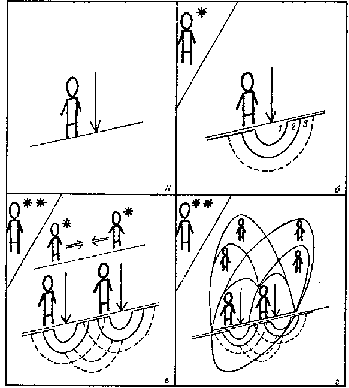
\includegraphics[width=.5\textwidth]{activity-nature-system.png}
\end{center}

Следует предположить, что ядро экологической ситуации задаётся фактом
столкновения нескольких различных систем деятельности на одном природном
ареале или одном участке природного материала. Отправной точкой при анализе
экологической ситуации является структура деятельности, сознательно
направленная или нецеленаправленно влияющая на природу. В схеме такая
структура деятельности может быть условно обозначена знаком «позиции» и знаком
«воздействия» на природный материал (смотри рисунок). Каждая позиция
характеризуется своими специфическими ценностями, целями, установками,
средствами, методами, способами мышления и деятельности. Позиция не может быть
сведена только к различию средств, хотя каждая позиция может быть
охарактеризована определённым представлением объекта и, следовательно,
определённой комбинацией средств деятельности. Однако отдельные средства могут
переходить и переходят из одной позиции в другую. 

Позиция, таким образом, задаётся особым пересечением многих отношений: прежде
всего, своей ориентированностью на практику особого типа, а следовательно,
возможными способами употребления знания. Принцип направленности знания на тот
или иной тип деятельности и своеобразной подчинённости знания практике того
или иного типа позволяет изображать структуры деятельности с помощью
графических знаков-символов — «позиций». 

Однако сам факт воздействия на природный материал со стороны тех или иных
источников деятельности ещё не создаёт экологической ситуации. Необходимым
элементом ситуации является рефлективная позиция, позиция внешнего наблюдателя
— изобразим её «позицией со звездочкой» (смотри рисунок 1б). Именно в этой
позиции «внешнего», стороннего наблюдателя и аналитика фиксируются последствия
воздействия на природный материал. Первая постановка экологической проблемы
связана с тем, что внешний наблюдатель начинает говорить от имени Природы; он
выделяет последствия отдельных воздействий на окружающую среду и делает
центральным моментом анализа факты рассогласования и расхождения между целями
искусственно-технического действия и результатами реального влияния на
Природу. 

При этом, если в истории становления и оформления экологической точки зрения
реальные наблюдатели — от Марша и чикагской школы экологии города до авторов
Римского клуба — лишь постепенно поднимались от непосредственного и
феноменального видения локальных последствий антропогенного воздействия на
окружающую среду к анализу глубинных и долговременных последствий
научно-технической революции в целом, на схеме простейшей экологической
ситуации мы будем фиксировать по крайней мере три «зоны» последствий. Первая
зона — контролируемых и учитываемых последствий, вторая — неконтролируемых, но
учитываемых последствий и третья — неконтролируемых и неучитываемых
последствий.  Характеристики «контролируемости» и «учитываемости» относятся
соответственно к самому действию и его рефлективному сопровождению.

Введённая схематизация имеет большой смысл в плане критики существующих
подходов: из неё, в частности, следует, что все те школы и направления,
которые работают только с учитываемыми, прогнозируемыми последствиями,
заведомо неправильно представляют структуру экологической ситуации и работают
на переупрощённых схемах объектов. Выделенные «зоны» фиксируют функциональную
структуру пространства последствий, и в этом плане неконтролируемые и
неучитываемые последствия оказываются принципиально «учтёнными» за счёт
использования такого рода изображения-схемы экологической ситуации. 

Однако структура экологической ситуации была бы принципиально неполной, если
бы мы остановились на введённых представлениях. Конституирующим моментом
ситуации является «появление» другой структуры деятельности, локализованной на
том же природном ареале. В этом случае «последствия» первого воздействия
должны рассматриваться как «условия» для развёртывания другой
деятельности. Если на одном природном материале замкнуто несколько различных
типов и форм деятельности, принципиально изменяется картина
последствий. Последствия, вызванные новой системой воздействий,
«накладываются» на исходную функциональную структуру последствий (смотри
рисунок 1в), возникает «интерференция», сдвигаются и меняются границы «зоны»
учитываемых и неучитываемых последствий. Возникает и ширится цепь «вторичных»
экологических эффектов. 

В том случае если на одном природном материале развёртываются две или
несколько различных структур деятельности, следует учитывать и анализировать,
помимо последствий воздействия на природный материал, также: 1) последствия
воздействия одних структур деятельности на другие структуры через
непосредственный деятельностный контекст; 2) последствия воздействия на другие
структуры деятельности через посредство «захваченного» и изменённого
природного материала (который в этом случае выступает как передаточное звено);
3) последствия воздействия на природный материал через изменения и
трансформацию «соседних» структур деятельности. При этом центр экологической
ситуации, естественно, сдвигается с отношения «деятельность — природа» на
отношение «деятельность 1 — деятельность 2»; возникает ряд новых конфликтов и
противоречий между структурами и системами деятельности, «паразитирующими» на
одном природном материале. 

Если на первых шагах развёртывания экологической ситуации мы имели дело с
последствиями как ответным «ударом» Природы, то теперь мы имеем дело с
последствиями, отраженными и преломлёнными сквозь призму «видения» и
деятельностного интереса других участников ситуации, других позиций и других
типов деятельности. «Кислотные дожди» выпадают на территории соседнего
государства, и возникает интернациональный конфликт. Выбросы газодобывающего
комплекса губят посевы риса, и возникает столкновение между двумя
министерствами. Загрязнение воздуха приводит к увеличению числа легочных
заболеваний, и Минздрав предъявляет претензии производственным объединениям
города. При этом провести границу между ситуацией взаимодействия различных
типов деятельности друг с другом и ситуацией воздействия на природное
окружение чрезвычайно трудно. Весь комплекс рассогласований и противоречий в
организации и соорганизации деятельности как бы «втягивается» в экологическую
ситуацию и кардинально изменяет её контуры. 

Наиболее важными компонентами экологической ситуации становятся: структуры
организации и управления (смотри рисунок 1г), конфликты между различными
структурами деятельности и их управленческими «надстройками» по вопросу о
преимущественных формах использования и употребления природного
материала. Каждая структура деятельности постоянно сталкивается с тем, что на
её систему употребления природного материала оказывает воздействие другая
деятельность. «Что вы делаете с Природой?» — вопрошают одни. Однако понимать
это каждый раз следует иначе: «Почему вы не даёте мне использовать и губить
Природу гораздо «прогрессивнее?» И в этом хоре голосов, звучащих в современной
экологической ситуации, голоса сторонних наблюдателей, говорящих от имени
Природы, смешиваются и переплетаются с голосами тех, кто говорит от лица
Деятельности — заинтересованно, преследуя свои специфические, в частности
ведомственные, цели и задачи. И при этом те, кто сегодня присваивают себе
право говорить от имени Природы с точки зрения «высших ценностей», точно так
же должны проходить специальную и тщательную «проверку», на какой тип
ценностей и целей они при этом ориентированы и на какой тип практики в
результате развёртывания этих ценностей можно выйти? 

Так усложняется структура экологической ситуации. Фиксируя на схеме лишь
символы позиций, мы позволяем читателю реконструировать и додумывать те
реальные противоречия и конфликты, свидетелями которых он сегодня
является. Вместе с тем мы предоставляем ему свободу в продолжении этой
«позиционной игры»: можно последовательно вводить в заданное схематическое
изображение новые позиции, усложняя схему и захватывая все новые и новые
пласты реальной ситуации. Здесь могут появиться учёные-алармисты,
ориентированные на конкретные проявления последствий — загрязнение воздуха,
воды, кризис городской среды; здесь появятся представители альтернативных
экологических движений со своими политическими интересами, которые заставляют
их, эксплуатируя второстепенные экологические эффекты, придавать им новое
звучание и статус всемирной проблемы; сюда должны быть включены представители
различных организационно-управленческих надстроек — начиная с министерств и
ведомств, со своими специфическими интересами и выработанным отношением к
ситуации на «местах», и кончая органами территориального и регионального
управления, использующими экологическую ситуацию для проведения политики
децентрализации и влияния на структуры отраслевого руководства. 

Вместе с тем проведённый анализ наглядно демонстрирует, что экологическая
ситуация есть прежде всего социальная и деятельностная ситуация. Не
реконструируя тех аспектов ситуации, где экологические вопросы и последствия
становятся средством политической борьбы и управления, организационного
влияния и прямого принуждения, где развёртываются столкновения и конфликты
между различными типами деятельности, нельзя понять сути и существа
экологической ситуации. Это хорошо и более подробно показано на примере
урбанистической ситуации в работе Е. Епишина «Программа «экополис» (ЧиП, 1986,
№ 9). Не видя существующих сегодня тенденций в области организации и
управления различными системами деятельности, паразитирующими на одном
природном материале, нельзя выделять структуру и границы экосистем. Нельзя не
понимать и того факта, что одни управляющие структуры направлены только на
соорганизацию различных типов деятельности, а другие, напротив, включают в
объект своего управления сам природный материал и выделенные зоны
последствий. 

В одном случае мы будем иметь дело с компромиссной экологией. В другом случае
мы вынуждены анализировать возможности и допустимые способы использования
природного материала; рассматривая организацию деятельности, мы должны
задаваться вопросом: какие формы использования природного ареала мы закрываем,
принимая то или иное стратегическое решение, какие формы использования стали
невозможными? Опираясь на понятия ресурса, территории, условий, мы
осуществляем альтернативное проектирование и прожектирование таких технологий
и систем деятельности, которых сегодня ещё нет. И тогда «природное», анализ
последствий и экологической ситуации становятся лишь моментом альтернативной
проектировочной работы, а вместе с тем ведут к программированию развития ДПС.

\begin{center}
  * * *
\end{center}

Таким образом, мы ввели простейшую схему экологической ситуации и наметили
пути её развёртывания. Значит ли это, что мы задали структуру ДПС? Нет. Пока
задано лишь то объектно-онтологическое поле, тот «фон», на котором могут быть
«прорисованы», «вырезаны» деятельностно-природные системы разного уровня
сложности. Границы различных ДПС будут определяться тем, какую практическую
рамку мы примем и под каким «углом зрения» будет выделяться центральный
системообразующий фактор и основной процесс, конституирующий целостность
данной ДПС.

Начиная говорить о ДПС, исследователи и проектировщики уверяют нас, что ДПС
состоит из двух подсистем: деятельностной и природной. Тем самым, применяя
структурные методы анализа, они восстанавливают методологический дуализм и
вводят ряд громоздких и в силу принятой постановки неразрешимых проблем. В XIX
веке такого же рода наивная метафизика привела к возникновению и широкому
распространению проблематики соотношения «души» и «тела». Сегодня мы понимаем,
что, до тех пор пока мы будем делить техническую работу с человеком на
практику работы с его физиологией и практику работы с его психологией, до тех
пор будут существовать психофизическая и психофизиологическая проблемы. Не
стоит повторять в области хозяйства тех логических и методологических ошибок,
которые делали психологи прошлого столетия. Принимая напрокат наивную
«метафизику природы» и противопоставляя «техническую» подсистему природной, мы
порождаем целый ряд псевдопроблем и ложных решений, по сути дела, закрывая
себе возможность выйти на реальное проектирование и исследование ДПС. 

ДПС есть единая система, и она не может быть «разрезана» на две или несколько
подсистем. По сути дела, идеология системного подхода и утверждает, что
рассматриваемый объект не может быть разделён на части и подсистемы, а должен
браться как одно, единое. 

Введённое схематическое изображение экологической ситуации фиксирует тот факт,
что структуры деятельности «захватывают» материал природы, трансформируют и
перерабатывают его особым образом, частично ассимилируют его, а частично
преобразовывают в соответствии с характером антропогенного и техногенного
воздействия. 

Однако выход к тем типам материала, которые не соответствуют форме,
противостоят ей реально-практически, есть по сути дела, первый ход к
совершенно иной, не материальной трактовке природного материала. Материал в
этом повороте сам выступает как полная система, живущая по своим законам и
имеющая свои специфические процессы. Другими словами, не форма противостоит
материалу, а одни процессы, конституирующие полную деятельностную, техническую
систему, противостоят другим процессам, конституирующим другую полную систему.
Вместо достаточно простой и очевидной категории «форма-материал» мы вынуждены
обращаться к гораздо более сложным категориям системного подхода.
«Система-кентавр» является в методологическом плане полисистемой, в рамках
которой одни процессы и системы становятся материалом, на котором
развёртываются другие процессы и специфические для них функциональные
структуры.

Центр тяжести системного анализа переносится на выявление различных способов
«зашнуровки» деятельностных и природных, естественно-исторических процессов,
на анализ механизмов «обискусствления» природных и «оестествления» технических
компонент, на проработку дополнительных категорий условия, последствия,
ресурса, границы и других. 

Отказываясь от ходячего представления о природе, принимая установку новой
концепции «второй природы» и новой «концепции рациональности», применимой к
«системам-кентаврам», мы закономерно должны ставить вопрос в его практическом
и логико-методо\-логическом повороте более широко. Необходимо привлекать иные,
более сложные системные категории и рассматривать не только и не столько
категориальные оппозиции «часть — целое», «элемент — связь», «форма —
материал», сколько отношения «процесс — материал», «функция — морфология»,
«процесс — структура», связи и соотношения между процессуальным,
структурно-функциональным, морфологическим и «материальным» представлением
сложной системы. Задачи приложения системной методологии при анализе
экологической ситуации наглядно демонстрируют дефицит наличных представлений;
задание онтологических картин техноприродного мира ставит и новые задачи перед
системным подходом. 

Вместе с тем, для того чтобы перейти к выделению «полных» ДПС, необходимо
теперь из позиции внешнего наблюдателя перейти в позицию организации и
действия по отношению ко всей конфигурации разных деятельностей с природным
материалом. Не занимая деятельностной позиции по отношению к экологической
ситуации, можно говорить об экологической обстановке, но нельзя проектировать
и исследовать ДПС. Напротив, принимая ту или иную практическую организационную
позицию, можно выделить и задать тот или иной основной «базовый» процесс и
соответствующие ему функциональные структуры и границы ДПС. «Вырезание» полных
систем в теории невозможно в чисто абстрактном залоге; лишь создавая ДПС и
выделяя «работающие» принципы управления, можно разрешать экологические
ситуации. 

А экология в этом новом повороте аккумулирует в себе практические мотивы
современной ситуации и обеспечивает превращение техники и поэзии прогресса в
практику строительства жизни и развития жизнедеятельности и мы еле
деятельности людей. 

В этом направлении мы сделали лишь несколько первых шагов, на каждом
сталкиваясь с мифами и призраками научного и обыденного сознания, с идолами
«площади» и идолами «рынка», на значение которых указывал ещё Ф. Бэкон. Быть
может, нам удастся среди разнообразия и пестроты точек зрения, в хаосе мнений
и программ нащупать тот путь, которым может и должна идти экология нового
столетия. 

\section{Библиография} 	
\begin{enumerate}
\item Андерсен Дж. М. Экология и науки об окружающей среде: биосфера,
  экосистемы, человек. — М., «Мысль», 1985.
\item Анучин В. А. Основы природопользования. Теоретический аспект. — М.,
  «Наука», 1987.
\item Глазычев В. Л. Социально-экологическая интерпретация городской среды. —
  М., «Наука», 1984.
\item Епишин В. К. Три методологических подхода в современной геологии.
  Системо-мыследеятельностный подход: понятие «геосистемы». // В сборнике:
  Системно-геологические исследования литосферы. — М., 1985.
\item Епишин В. К., Епишин Е. В. Геология как сфера деятельности
  (системно-аксио\-логический подход). // В сборнике: Системные исследования и
  разработки в геологии. — М., МОИП, 1985.
\item Епишин Е. В. Программа «экополис». — Человек и природа. — 1986. — № 9.
\item Епишин Е. В. Авариеведение. — Человек и природа. — 1987. — № 8.
\item Ойзерман М. Т., Рац М. В., Щедровицкий Г. П. Научные и практические
  вопросы создания эффективно реализуемых проектов с точки зрения изысканий.
  // В сборнике: Прометодологии и технологии инженерных изысканий. — М., 1985.
\item Сен-Марк Ф. Социализация природы. — М., «Прогресс», 1977.
\item Фёдоров В. Д., Гильмаиов Т. Б. Экология. — М., МГУ, 1980.
\item Щедровицкий Г. П. Проблемы методологии системного исследования. — М.,
  Знание, 1964.
\item Щедровицкий Г. П. Принципы и общая схема методологической организации
  сис\-темно-структурных исследовании и разработок. // Ежегодник «Системные
  исследования». — М., «Наука», 1981.
\end{enumerate}


\end{document}
